% Generated by scripts/build_performance.py; edit the structured sources.
\subsection{What is reported, and what is missing}
The five selected systems have sparse coverage across the selected benchmark families (Figure~\ref{fig:performance-coverage}). Missing results are NR, not zero. FLAIR's separate study evaluations below do not fill an FDB-v3 or SRQA cell. Source versions, table/page locators and PDF hashes are archived alongside the reported values; these checks verify transcription, not experimental reproduction.
\begin{figure}[H]
\centering
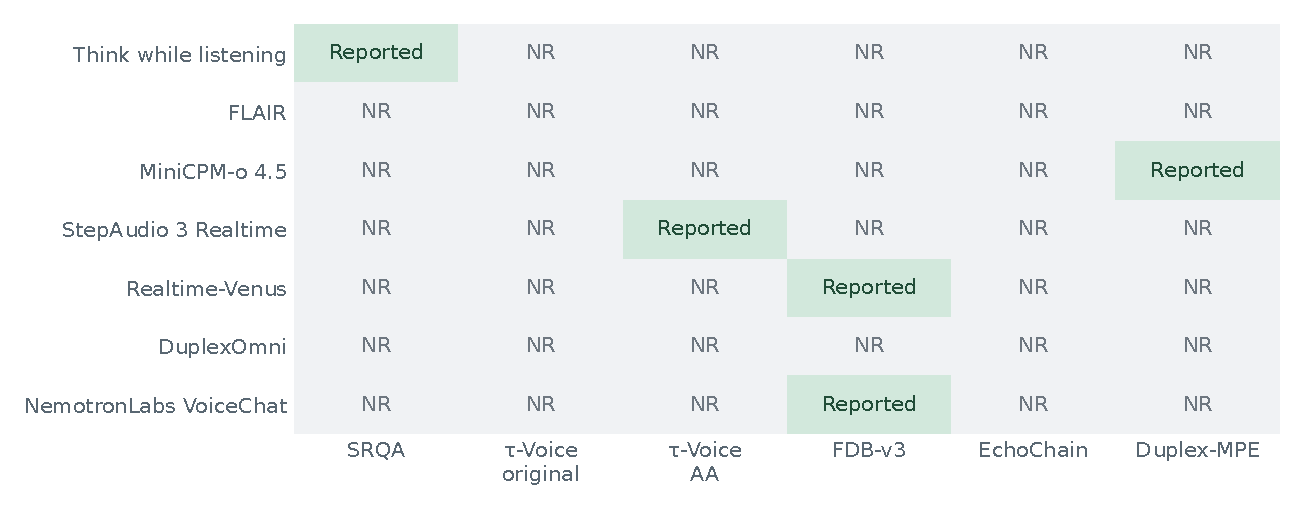
\includegraphics[width=\linewidth]{figures/performance/coverage.pdf}
\caption{Reported selected-system coverage in the five benchmark families, with the two $\tau$-Voice implementations kept separate. NR means no matching result was located in the reviewed sources.}
\label{fig:performance-coverage}
\end{figure}
\paragraph{How to read the profiles.}
Radars show raw percentages on a shared 0--100 scale within one protocol; their area is not a model score. Separate bars are used for mixed units or fewer than three metrics. Solid lines denote selected configurations; dashed lines denote reference/ablation configurations. Compare named curves and individual metrics, not polygon area or panels from different benchmarks. No missing cell is imputed and no cross-benchmark average is calculated. The figures use source-reported point estimates, without reproducing experiments or inventing uncertainty bars.
Closed references are benchmark-source leaders where reported, not current global SoTA. SRQA and Duplex-MPE do not test a closed voice system. FLAIR's historical interaction table contains only one closed API reference, with no precise revision. Imported reference scores and later system-report evaluations are not a common rerun.
\clearpage
\subsection{Think while listening: SRQA}
Two TWL-study checkpoints are distinct. Kimi-Audio is a speech reference, not a full-duplex system. The table also includes Qwen2-Audio; Helium's non-comparable text result is omitted. \citep{thinklisten}
\begin{figure}[H]
\centering
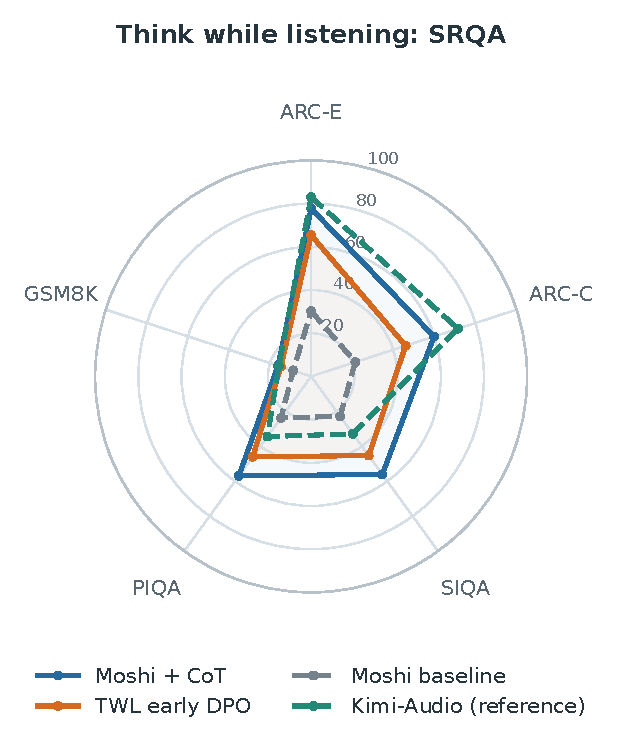
\includegraphics[width=0.78\linewidth]{figures/performance/twl.pdf}
\caption{Think while listening: SRQA. Raw percentages; higher is better. Exact values and additional context references are in the adjacent table.}
\label{fig:performance-twl}
\end{figure}
% Generated by scripts/build_performance.py; edit research/reported-performance.json.
\begin{table}[H]
\centering\small
\setlength{\tabcolsep}{3pt}
\setlength{\tablewidth}{\dimexpr\linewidth-10\tabcolsep\relax}
\renewcommand{\arraystretch}{1.06}
\caption{SRQA. Percent; higher is better. Bold: best among the displayed references, not a source-wide or current SoTA. \citep{thinklisten}}
\label{tab:performance-srqa}
\begin{tabular}{@{}>{\raggedright\arraybackslash}p{0.32\tablewidth}>{\centering\arraybackslash}p{0.136000\tablewidth}>{\centering\arraybackslash}p{0.136000\tablewidth}>{\centering\arraybackslash}p{0.136000\tablewidth}>{\centering\arraybackslash}p{0.136000\tablewidth}>{\centering\arraybackslash}p{0.136000\tablewidth}@{}}
\toprule
\textbf{Model / configuration} & \textbf{ARC-E} & \textbf{ARC-C} & \textbf{SIQA} & \textbf{PIQA} & \textbf{GSM8K} \\
\midrule
\textbf{Moshi + CoT (TWL study)} & 77.7 & 59.8 & \textbf{56.1} & \textbf{56.9} & 16.1 \\
\textbf{TWL: early length-DPO} & 65.4 & 46.0 & 45.3 & 46.0 & 14.7 \\
Moshi baseline & 30.2 & 21.5 & 22.8 & 23.8 & 8.7 \\
Kimi-Audio-7B-Instruct & \textbf{83.0} & \textbf{71.5} & 32.9 & 34.4 & 15.7 \\
Qwen2-Audio-7B-Instruct & 59.1 & 42.4 & 21.9 & 24.5 & \textbf{18.1} \\
\bottomrule
\end{tabular}
\end{table}

{\small\textbf{Reading this profile (review interpretation).} The CoT configuration is stronger on these tasks than foundation Moshi, but early length-DPO is a different accuracy/latency operating point, not the same high-accuracy checkpoint.}
\clearpage
\subsection{FLAIR: spoken QA accuracy}
FLAIR's own QA suite is not SRQA. Only accuracy-valued tasks are plotted; 1–5 open-ended judge scores are excluded. Published reference scores are imported, not all rerun. Kimi-Audio is half-duplex. \citep{flair}
\begin{figure}[H]
\centering
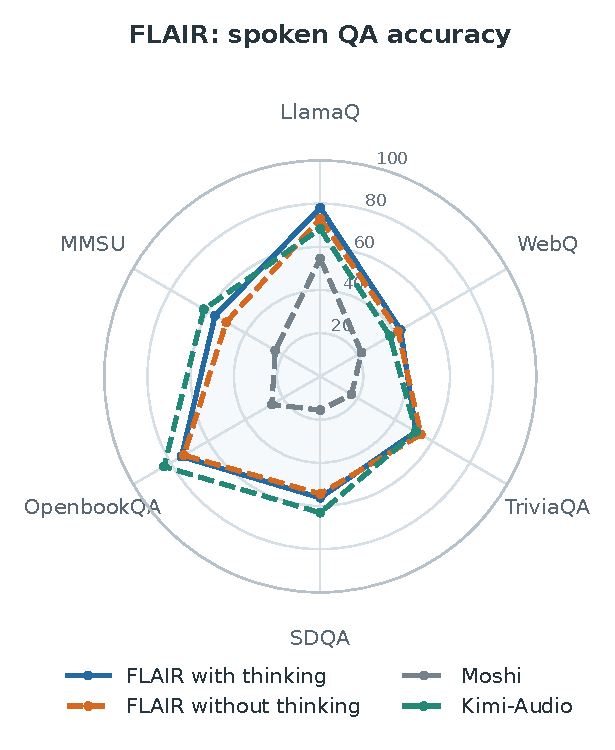
\includegraphics[width=0.78\linewidth]{figures/performance/flair-qa.pdf}
\caption{FLAIR: spoken QA accuracy. Raw percentages; higher is better. Exact values and additional context references are in the adjacent table.}
\label{fig:performance-flair-qa}
\end{figure}
% Generated by scripts/build_performance.py; edit research/reported-performance.json.
\begin{table}[H]
\centering\small
\setlength{\tabcolsep}{3pt}
\setlength{\tablewidth}{\dimexpr\linewidth-12\tabcolsep\relax}
\renewcommand{\arraystretch}{1.06}
\caption{FLAIR study: spoken QA. Percent; higher is better. Bold: best among the displayed references, not a source-wide or current SoTA. \citep{flair}}
\label{tab:performance-flair_qa}
\begin{tabular}{@{}>{\raggedright\arraybackslash}p{0.32\tablewidth}>{\centering\arraybackslash}p{0.113333\tablewidth}>{\centering\arraybackslash}p{0.113333\tablewidth}>{\centering\arraybackslash}p{0.113333\tablewidth}>{\centering\arraybackslash}p{0.113333\tablewidth}>{\centering\arraybackslash}p{0.113333\tablewidth}>{\centering\arraybackslash}p{0.113333\tablewidth}@{}}
\toprule
\textbf{Model / configuration} & \textbf{LlamaQ} & \textbf{WebQ} & \textbf{TriQA} & \textbf{SDQA} & \textbf{OBQA} & \textbf{MMSU} \\
\midrule
\textbf{FLAIR w/ thk} & \textbf{78.0} & \textbf{43.0} & 51.2 & 56.2 & 74.2 & 56.2 \\
FLAIR w/o thk & 73.0 & 41.7 & \textbf{53.8} & 54.4 & 72.9 & 50.2 \\
Moshi & 54.5 & 22.1 & 16.7 & 15.6 & 25.9 & 24.0 \\
Freeze-Omni & 56.2 & 27.9 & 28.5 & 53.5 & 31.0 & 28.1 \\
Kimi-Audio & 68.3 & 37.3 & 51.2 & \textbf{63.1} & \textbf{83.5} & \textbf{62.2} \\
\bottomrule
\end{tabular}
\end{table}

{\small\textbf{Reading this profile (review interpretation).} Latent thinking improves several tasks over the no-thinking ablation, but not every task: TriviaQA is lower. No single curve wins across all tasks shown.}
\clearpage
\subsection{FLAIR: earlier duplex interaction suite}
Separate axes preserve percentages, seconds and 0–5 judge scores. TOR means takeover rate. Gemini Live is the study's sole closed reference; its API revision is unspecified. This is not FDB-v3 tool use. \citep{flair}
\begin{figure}[H]
\centering
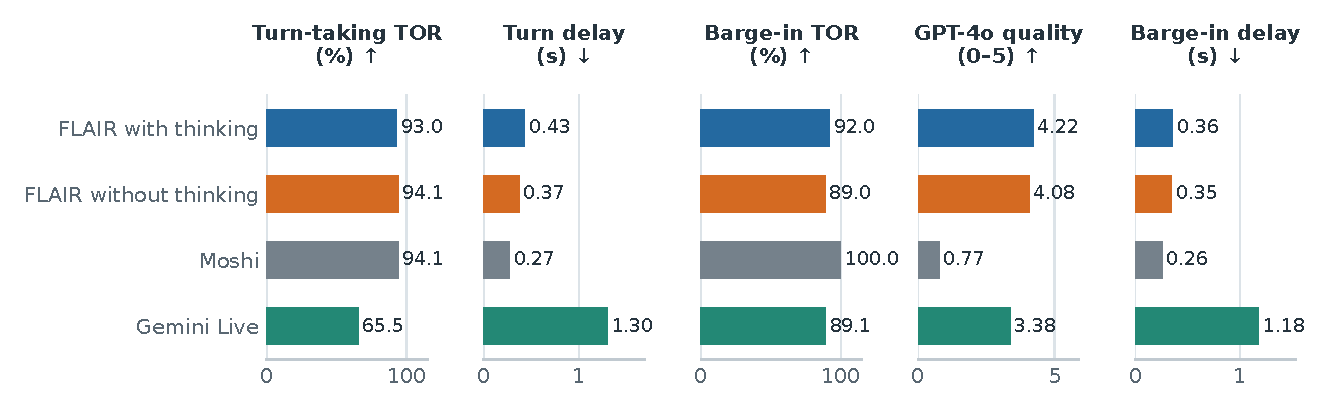
\includegraphics[width=\linewidth]{figures/performance/flair-interaction.pdf}
\caption{FLAIR: earlier duplex interaction suite. Units and directions are labeled per panel. Exact values and additional context references are in the adjacent table.}
\label{fig:performance-flair-interaction}
\end{figure}
% Generated by scripts/build_performance.py; edit research/reported-performance.json.
\begin{table}[H]
\centering\small
\setlength{\tabcolsep}{3pt}
\setlength{\tablewidth}{\dimexpr\linewidth-10\tabcolsep\relax}
\renewcommand{\arraystretch}{1.06}
\caption{FLAIR study: Full-Duplex-Bench (original suite). Each column states its unit and direction. Bold: best among the displayed references, not a source-wide or current SoTA. \citep{flair}}
\label{tab:performance-flair_interaction}
\begin{tabular}{@{}>{\raggedright\arraybackslash}p{0.32\tablewidth}>{\centering\arraybackslash}p{0.136000\tablewidth}>{\centering\arraybackslash}p{0.136000\tablewidth}>{\centering\arraybackslash}p{0.136000\tablewidth}>{\centering\arraybackslash}p{0.136000\tablewidth}>{\centering\arraybackslash}p{0.136000\tablewidth}@{}}
\toprule
\textbf{Model / configuration} & \textbf{Turn-taking TOR (\%; higher)} & \textbf{Turn-taking latency (s; lower)} & \textbf{Barge-in TOR (\%; higher)} & \textbf{Barge-in GPT-4o (0–5; higher)} & \textbf{Barge-in latency (s; lower)} \\
\midrule
\textbf{FLAIR w/ thk} & 93.0 & 0.43 & 92.0 & \textbf{4.22} & 0.36 \\
FLAIR w/o thk & \textbf{94.1} & 0.37 & 89.0 & 4.08 & 0.35 \\
Moshi & \textbf{94.1} & \textbf{0.27} & \textbf{100.0} & 0.77 & \textbf{0.26} \\
Gemini Live & 65.5 & 1.30 & 89.1 & 3.38 & 1.18 \\
\bottomrule
\end{tabular}
\end{table}

{\small\textbf{Reading this profile (review interpretation).} Response quality, takeover rate and response delay expose different trade-offs. A high takeover rate alone does not establish a useful answer.}
\clearpage
\subsection{StepAudio 3 Realtime: $\tau$-Voice (AA)}
Artificial Analysis implementation and API versions from StepAudio's report. The radar shows three domain success rates; the bar panel shows the separately reported equal-domain macro. Grok is the macro leader, not the winner in every domain. \citep{step3}
\begin{figure}[H]
\centering
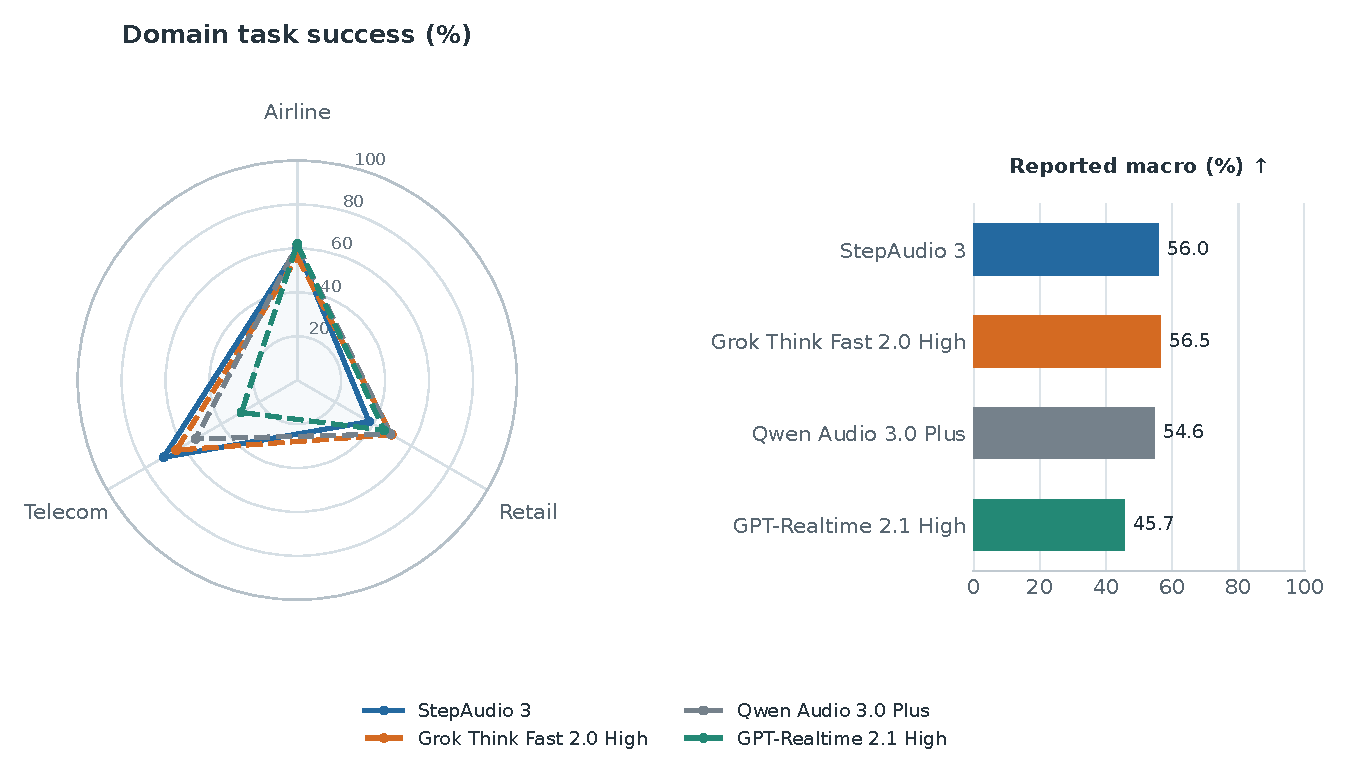
\includegraphics[width=\linewidth]{figures/performance/step3.pdf}
\caption{StepAudio 3 Realtime: $\tau$-Voice (AA). Raw percentages; higher is better. Exact values and additional context references are in the adjacent table.}
\label{fig:performance-step3}
\end{figure}
% Generated by scripts/build_performance.py; edit research/reported-performance.json.
\begin{table}[H]
\centering\small
\setlength{\tabcolsep}{3pt}
\setlength{\tablewidth}{\dimexpr\linewidth-8\tabcolsep\relax}
\renewcommand{\arraystretch}{1.06}
\caption{$\tau$-Voice (AA). Percent; higher is better. Bold: best among the displayed references, not a source-wide or current SoTA. \citep{step3}}
\label{tab:performance-tau_aa}
\begin{tabular}{@{}>{\raggedright\arraybackslash}p{0.32\tablewidth}>{\centering\arraybackslash}p{0.170000\tablewidth}>{\centering\arraybackslash}p{0.170000\tablewidth}>{\centering\arraybackslash}p{0.170000\tablewidth}>{\centering\arraybackslash}p{0.170000\tablewidth}@{}}
\toprule
\textbf{Model / configuration} & \textbf{Airline} & \textbf{Retail} & \textbf{Telecom} & \textbf{Macro task success} \\
\midrule
\textbf{StepAudio 3 Realtime} & 60.0 & 37.7 & \textbf{70.2} & 56.0 \\
Grok Voice Think Fast 2.0 High & 56.0 & \textbf{49.7} & 63.7 & \textbf{56.5} \\
Qwen Audio 3.0 Realtime Plus & 61.3 & 49.0 & 53.5 & 54.6 \\
GPT-Realtime-2.1 High & \textbf{62.0} & 45.6 & 29.4 & 45.7 \\
\bottomrule
\end{tabular}
\end{table}

{\small\textbf{Reading this profile (review interpretation).} The reported macro scores are close while the domain profiles differ. This comparison cannot be pooled with the original clean/realistic $\tau$-Voice results.}
\clearpage
\subsection{Realtime-Venus: Full-Duplex-Bench v3}
Both Venus frontends are from the revised system report; closed references are from the benchmark comparison. GPT-Realtime leads these three metrics in that source, not a current global leaderboard. This is not a common rerun. \citep{fdb3,venus}
\begin{figure}[H]
\centering
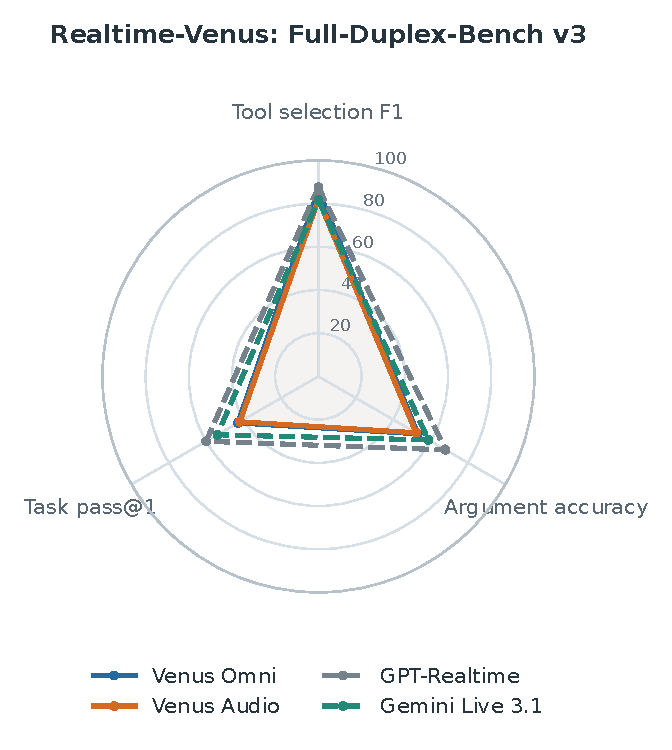
\includegraphics[width=0.78\linewidth]{figures/performance/venus.pdf}
\caption{Realtime-Venus: Full-Duplex-Bench v3. Raw percentages; higher is better. Exact values and additional context references are in the adjacent table.}
\label{fig:performance-venus}
\end{figure}
% Generated by scripts/build_performance.py; edit research/reported-performance.json.
\begin{table}[H]
\centering\small
\setlength{\tabcolsep}{3pt}
\setlength{\tablewidth}{\dimexpr\linewidth-6\tabcolsep\relax}
\renewcommand{\arraystretch}{1.06}
\caption{Full-Duplex-Bench v3. Percent; higher is better. Bold: best among the displayed references, not a source-wide or current SoTA. \citep{fdb3,venus}}
\label{tab:performance-fdb3}
\begin{tabular}{@{}>{\raggedright\arraybackslash}p{0.32\tablewidth}>{\centering\arraybackslash}p{0.226667\tablewidth}>{\centering\arraybackslash}p{0.226667\tablewidth}>{\centering\arraybackslash}p{0.226667\tablewidth}@{}}
\toprule
\textbf{Model / configuration} & \textbf{Tool F1} & \textbf{Argument accuracy} & \textbf{Pass@1} \\
\midrule
\textbf{Realtime-Venus-Omni} & 86.0 & 53.1 & 43.0 \\
\textbf{Realtime-Venus-Audio} & 82.0 & 52.2 & 42.0 \\
GPT-Realtime & \textbf{87.6} & \textbf{68.0} & \textbf{60.0} \\
Gemini Live 3.1 & 81.7 & 58.8 & 54.0 \\
\bottomrule
\end{tabular}
\end{table}

{\small\textbf{Reading this profile (review interpretation).} Tool-selection F1 is substantially higher than complete-task pass@1. These metrics have different success criteria, so their difference is not a stage-wise failure rate.}
\clearpage
\subsection{MiniCPM-o 4.5: Duplex-MPE}
Explicit and implicit addressing are separate panels. Moshi and Voila are representative speech references. Answer accuracy is conditional on fresh responses; yield uses model-specific eligible speaking events. Polygon area is not an overall score. Gemini's transcript control is excluded. \citep{mpe}
\begin{figure}[H]
\centering
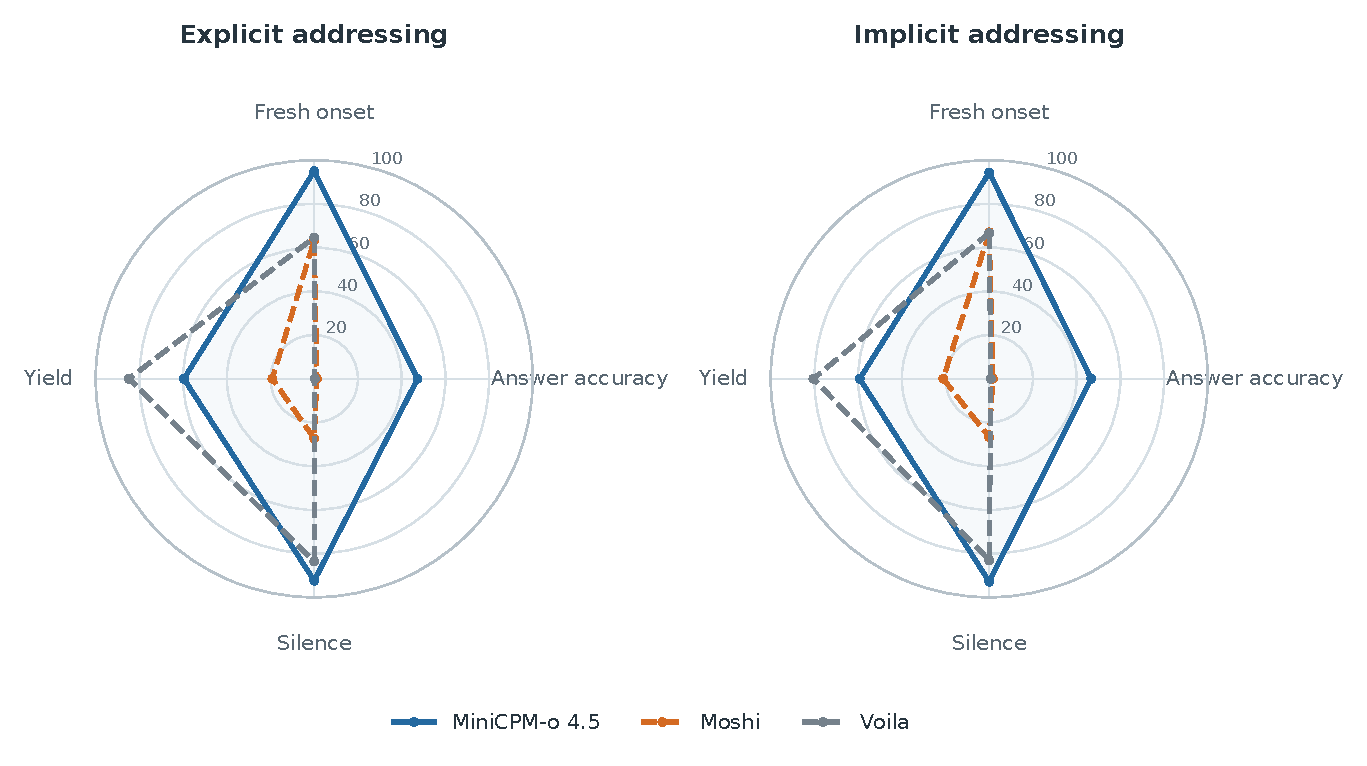
\includegraphics[width=\linewidth]{figures/performance/minicpm.pdf}
\caption{MiniCPM-o 4.5: Duplex-MPE. Raw percentages; higher is better. Exact values and additional context references are in the adjacent table.}
\label{fig:performance-minicpm}
\end{figure}
% Generated by scripts/build_performance.py; edit research/reported-performance.json.
\begin{table}[H]
\centering\small
\setlength{\tabcolsep}{3pt}
\setlength{\tablewidth}{\dimexpr\linewidth-8\tabcolsep\relax}
\renewcommand{\arraystretch}{1.06}
\caption{Duplex-MPE. Percent; higher is better. Bold: best among the displayed references, not a source-wide or current SoTA. \citep{mpe}}
\label{tab:performance-mpe}
\begin{tabular}{@{}>{\raggedright\arraybackslash}p{0.32\tablewidth}>{\centering\arraybackslash}p{0.170000\tablewidth}>{\centering\arraybackslash}p{0.170000\tablewidth}>{\centering\arraybackslash}p{0.170000\tablewidth}>{\centering\arraybackslash}p{0.170000\tablewidth}@{}}
\toprule
\textbf{Model / configuration} & \textbf{Fresh onset} & \textbf{Answer accuracy} & \textbf{Silence preservation} & \textbf{Yield} \\
\midrule
\textbf{MiniCPM-o 4.5 (explicit)} & \textbf{95.00} & \textbf{47.30} & 92.42 & 59.64 \\
\textbf{MiniCPM-o 4.5 (implicit)} & 94.35 & 46.65 & \textbf{92.89} & 59.25 \\
Voila (explicit) & 64.65 & 0.31 & 83.51 & \textbf{84.84} \\
Voila (implicit) & 66.70 & 0.75 & 83.07 & 80.46 \\
Moshi (explicit) & 63.40 & 1.23 & 27.34 & 19.18 \\
Moshi (implicit) & 67.00 & 1.70 & 26.76 & 21.07 \\
\bottomrule
\end{tabular}
\end{table}

{\small\textbf{Reading this profile (review interpretation).} MiniCPM-o combines frequent fresh responses and silence preservation, but conditional answer accuracy is much lower. Voila's higher yield is conditional on different eligible events.}
\clearpage
\subsection{Original $\tau$-Voice: closed voice references}
Original benchmark Table 6 All row; clean and realistic conditions remain separate. None of the five selected systems is evaluated here. GPT-5's text control is not plotted as a voice competitor. \citep{tauvoice}
\begin{figure}[H]
\centering
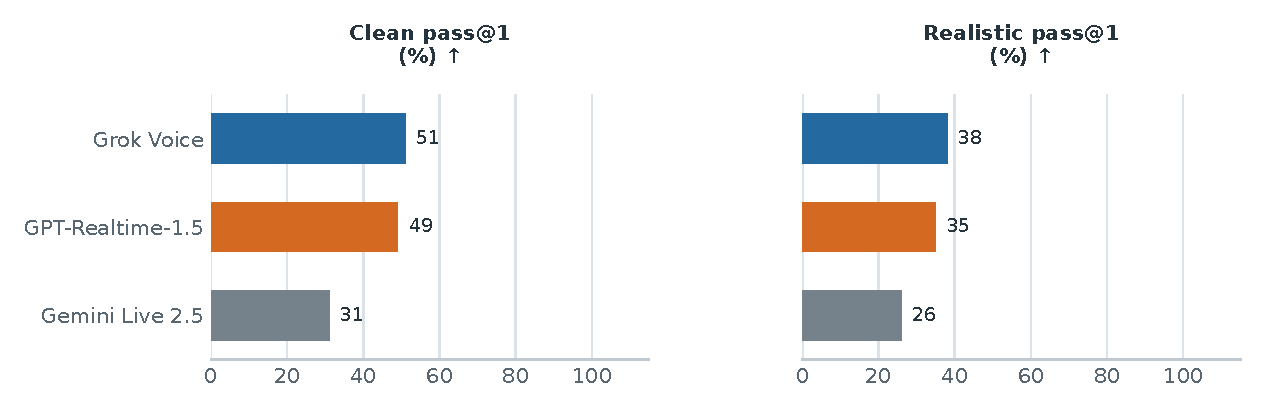
\includegraphics[width=\linewidth]{figures/performance/tau-original.pdf}
\caption{Original $\tau$-Voice: closed voice references. Units and directions are labeled per panel. Exact values and additional context references are in the adjacent table.}
\label{fig:performance-tau-original}
\end{figure}
% Generated by scripts/build_performance.py; edit research/reported-performance.json.
\begin{table}[H]
\centering\small
\setlength{\tabcolsep}{3pt}
\setlength{\tablewidth}{\dimexpr\linewidth-4\tabcolsep\relax}
\renewcommand{\arraystretch}{1.06}
\caption{$\tau$-Voice. Percent; higher is better. Bold: best among the displayed references, not a source-wide or current SoTA. \citep{tauvoice}}
\label{tab:performance-tau_original}
\begin{tabular}{@{}>{\raggedright\arraybackslash}p{0.32\tablewidth}>{\centering\arraybackslash}p{0.340000\tablewidth}>{\centering\arraybackslash}p{0.340000\tablewidth}@{}}
\toprule
\textbf{Model / configuration} & \textbf{Clean pass@1} & \textbf{Realistic pass@1} \\
\midrule
Grok Voice & \textbf{51} & \textbf{38} \\
GPT-Realtime-1.5 & 49 & 35 \\
Gemini Live 2.5 & 31 & 26 \\
\bottomrule
\end{tabular}
\end{table}

{\small\textbf{Reading this profile (review interpretation).} All three voice systems perform worse under realistic audio conditions in this source comparison; later $\tau$-Voice implementations are separate evidence.}
\clearpage
\subsection{EchoChain: closed voice references}
Paper Table 1, across 200 interrupted conversations. MPR requires every criterion in a conversation to pass; MCP scores individual criteria. None of the five selected systems is evaluated here. \citep{echochain}
\begin{figure}[H]
\centering
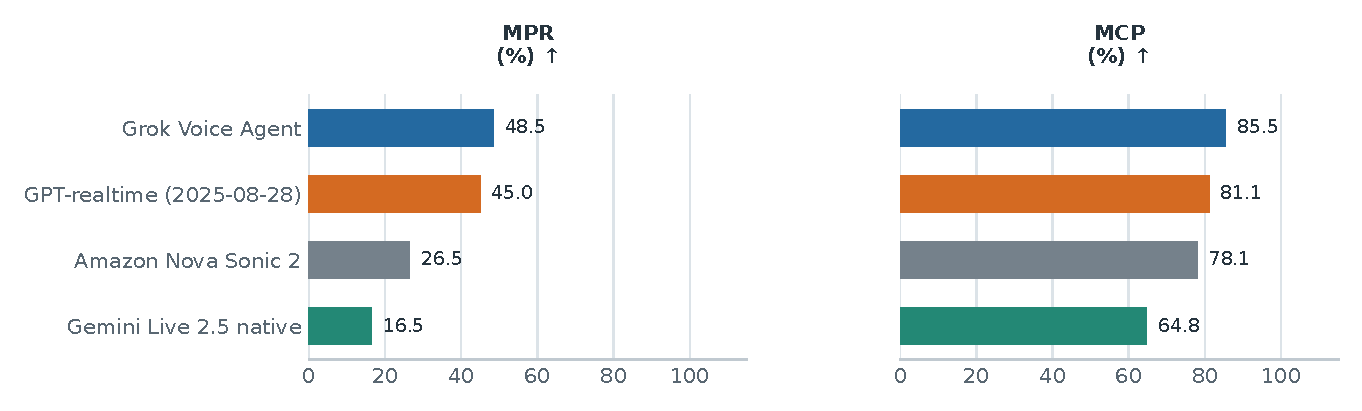
\includegraphics[width=\linewidth]{figures/performance/echochain.pdf}
\caption{EchoChain: closed voice references. Units and directions are labeled per panel. Exact values and additional context references are in the adjacent table.}
\label{fig:performance-echochain}
\end{figure}
% Generated by scripts/build_performance.py; edit research/reported-performance.json.
\begin{table}[H]
\centering\small
\setlength{\tabcolsep}{3pt}
\setlength{\tablewidth}{\dimexpr\linewidth-4\tabcolsep\relax}
\renewcommand{\arraystretch}{1.06}
\caption{EchoChain. Percent; higher is better. Bold: best among the displayed references, not a source-wide or current SoTA. \citep{echochain}}
\label{tab:performance-echo}
\begin{tabular}{@{}>{\raggedright\arraybackslash}p{0.32\tablewidth}>{\centering\arraybackslash}p{0.340000\tablewidth}>{\centering\arraybackslash}p{0.340000\tablewidth}@{}}
\toprule
\textbf{Model / configuration} & \textbf{MPR} & \textbf{MCP} \\
\midrule
Grok Voice Agent & \textbf{48.5} & \textbf{85.5} \\
GPT-realtime-2025-08-28 & 45.0 & 81.1 \\
Amazon Nova Sonic 2 & 26.5 & 78.1 \\
Gemini Live 2.5 native audio & 16.5 & 64.8 \\
\bottomrule
\end{tabular}
\end{table}

{\small\textbf{Reading this profile (review interpretation).} Passing many individual criteria does not guarantee complete conversation success. Even the strongest reported voice reference passes fewer than half of conversations.}
\paragraph{Text controls, not voice competitors.}
GPT-5 (reasoning, text): 85\% (Text task pass@1). Text control, not a realtime voice result. \citep{tauvoice}\par
Gemini 3.1 Pro (explicit, transcript): 94.70 / 90.39 / 95.37\% (Response presence / Conditional answer / Silence preservation). Table 17 reference run; not acoustic, not a speech-model upper bound. \citep{mpe}\par
Gemini 3.1 Pro (implicit, transcript): 30.40 / 79.11 / 99.34\% (Response presence / Conditional answer / Silence preservation). No fresh-onset or stopping score; speaker-attributed transcript is supplied. \citep{mpe}\par
